\documentclass[12pt, a4paper, oneside]{ctexbook}
\usepackage{amsmath, amsthm, amssymb, hyperref, mathrsfs}
% 引入超链接hyperref
\usepackage{bm}% 加粗公式内字体bm
\usepackage{graphicx} %插入图片的宏包
\usepackage{float} %设置图片浮动位置的宏包
\usepackage{subfigure} %插入多图时用子图显示的宏包

\graphicspath{{../images/}}


% 超链接样式
\hypersetup{hidelinks,colorlinks=true,allcolors=black,pdfstartview=Fit,breaklinks=true}

% 标题,作者,时间
\title{{\Huge{\textbf{工程数学基础}}}}
% \href{超链接地址}{文本}引入超链接
\author{\href{https://space.bilibili.com/230105574}{DR\_CAN}}
\date{\today}



% 定理,定义,引理,推论,命题,例
\linespread{1.5}
\newtheorem{theorem}{定理}[section]
\newtheorem{definition}[theorem]{定义}
\newtheorem{lemma}[theorem]{引理}
\newtheorem{corollary}[theorem]{推论}
\newtheorem{example}[theorem]{例}
\newtheorem{proposition}[theorem]{命题}



% ------------------------------------------------------------------------------
% 文章主体
\begin{document}
% 编译标题
\maketitle
% ------------------------------------------------------------------------------



% 章节目录
\newpage
\pagenumbering{Roman}
\setcounter{page}{1}
\tableofcontents
\newpage
\setcounter{page}{1}
\pagenumbering{arabic}


% 正文
% 章节
\chapter{特征值与特征向量}

% \bm{}加粗公式内文本
在数学中,特别是线性代数中,对于一个给定的线性变换$\bm{A}$,它的特征向量$\bm{v}$经过这个线性变换的作用之后,得到的新向量仍然与原来的$\bm{v}$保持在同一条直线上,但其长度或方向也许会改变,即

$$ \bm{Av}=\bm {\lambda v} $$


其中$\bm{\lambda}$为标量,即特征向量的长度在该线性变换下缩放的比例,称为其特征值


% 小节
\section{线性变化}

 现有二维线性变化矩阵

$$
\bm{A}=
 \left[
    \begin{matrix}
        1 & 1 \\
        4 & -2 \\
    \end{matrix}
 \right]
 $$

以及一个向量

$$\bm{v_1}=
\left[
    \begin{matrix}
        1 \\ 2 \\
    \end{matrix}
\right]
$$

向量$\bm{v_1}$通过$\bm{A}$的线性变换,即

$$
\bm{A v_1}=
\left[
    \begin{matrix}
        1 & 1 \\
        4 & -2 \\
    \end{matrix}
\right]
\left[
    \begin{matrix}
        1 \\ 2 \\
    \end{matrix}
\right]=
\left[
    \begin{matrix}
        1 \times 1 + 1 \times 2 \\
        4 \times 1 + (-2) \times 2 \\
    \end{matrix}
\right]=
\left[
    \begin{matrix}
        3 \\ 0 \\
    \end{matrix}
\right]
$$


笛卡尔坐标系下$v_1$向量的$A$变化如图\ref{md230213001}所示


\begin{figure}[H] 
    %H为当前位置,!htb为忽略美学标准,htbp为浮动图形
    \centering %图片居中
    % width=0.80\texwidth表示图片占页面的80%宽度
    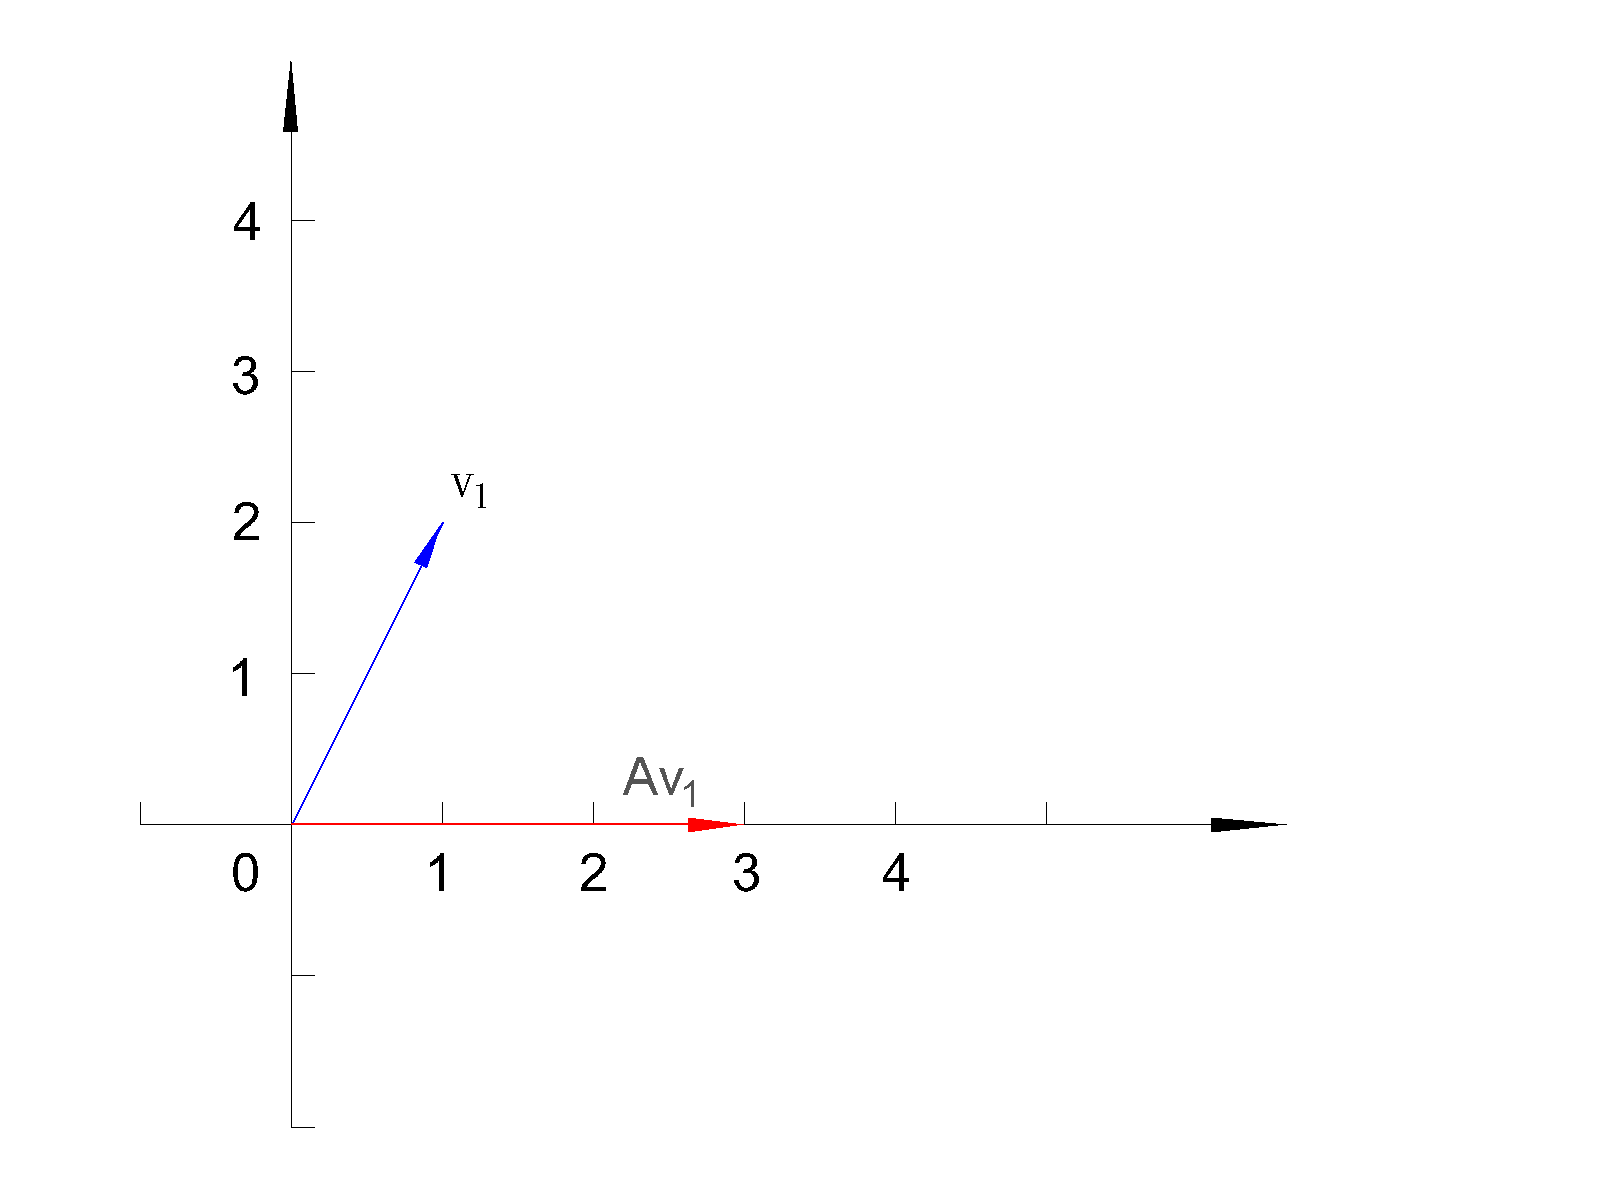
\includegraphics[width=0.80\textwidth]{md230213001.png}
    \caption{$v_1$向量的$A$变化} %图片标题
    \label{md230213001} %图片引用的标签
\end{figure}

通过图\ref{md230213001}可以看出$v_1$通过$A$的线性变化后大小和方向都发生了变化

现有另一个向量

$$
v_2=
\left[
    \begin{matrix}
        1 \\ 1 \\
    \end{matrix}
\right]
$$

同样的对$v_2$进行$A$线性变化得到

$$
Av_2=
\left[
    \begin{matrix}
        1 & 1 \\
        4 & -2 \\
    \end{matrix}
\right]
\left[
    \begin{matrix}
        1 \\ 1 \\
    \end{matrix}
\right]=
\left[
    \begin{matrix}
        1 \times 1 + 1 \times 1 \\
        4 \times 1 + (-2) \times 1 \\
    \end{matrix}
\right]=
\left[
    \begin{matrix}
        2 \\ 2 \\
    \end{matrix}
\right]=
2\left[
    \begin{matrix}
        1 \\ 1 \\
    \end{matrix}
\right]=
2v_2
$$

$Av_2$与$v_2$在一条直线上,根据定义可知$v_2$是矩阵$A$的特征向量,缩放比例2即是特征值$\lambda$

\begin{figure}[H]
    \centering
    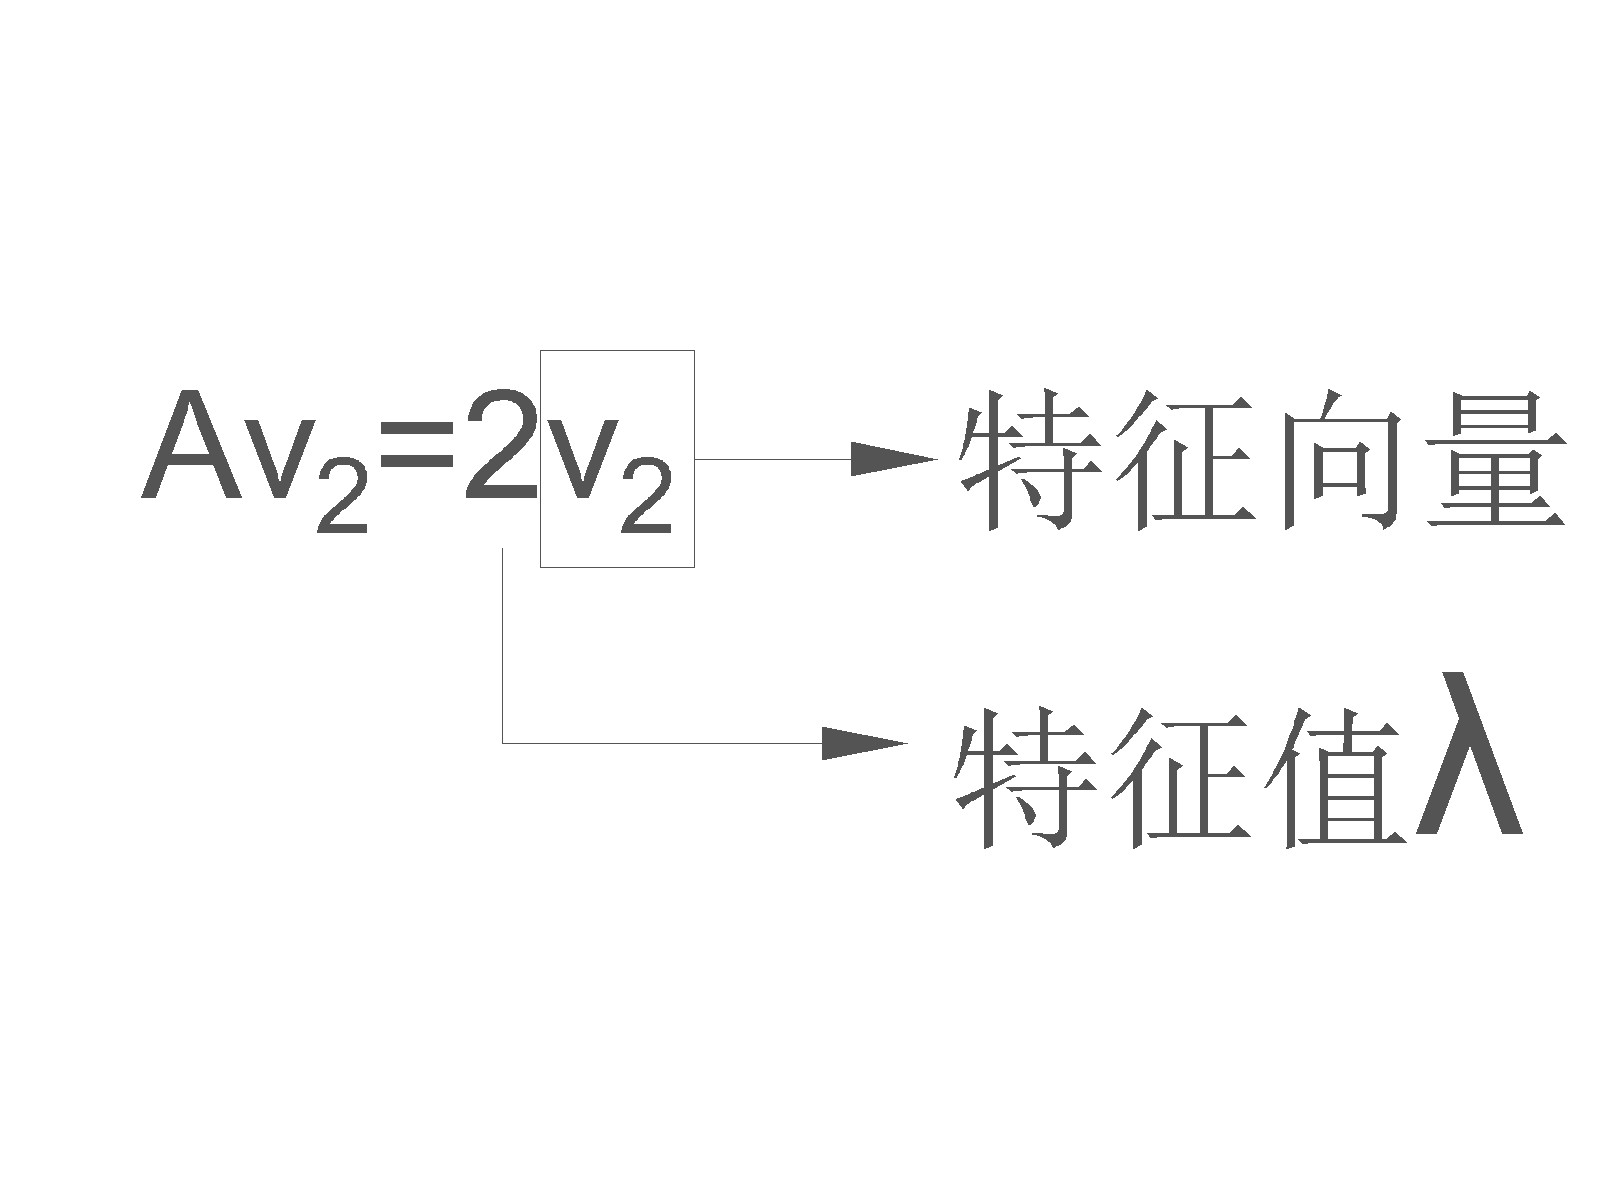
\includegraphics[width=0.3\textwidth]{md230215001.png}
    \label{md230215001}
\end{figure}

\section{求解特征值特征向量}

求解矩阵的特征值和特征向量推导:
\begin{equation}
    Av=\lambda v
\end{equation}
\begin{equation} 
    Av-\lambda v=0
\end{equation}
\begin{equation}\label{eq1}
    (A-\lambda I)v=0
\end{equation}

此处$I$是一个单位矩阵

若式\ref{eq1}有非零解则有

$$
\begin{vmatrix}
    A-\lambda I
\end{vmatrix}
=0
$$

通过上式即可求得特征值$\lambda$,然后再将特征值带回式\ref{eq1}中即可得到特征向量。




\end{document}
